\section{实验结果及分析}

\subsection{仿真波形}
图\ref{fig:wave}为单周期CPU行为仿真波形图，展示了CPU执行mipstest程序的完整过程。波形中pc信号按指令顺序递增，instr信号与coe文件中的机器码一致；rs（RD1）、rt（RD2）为寄存器堆读出值，rd为目的寄存器编号，result为写回结果，各信号变化与预期执行路径吻合。

\begin{figure}[htbp]
    \centering
    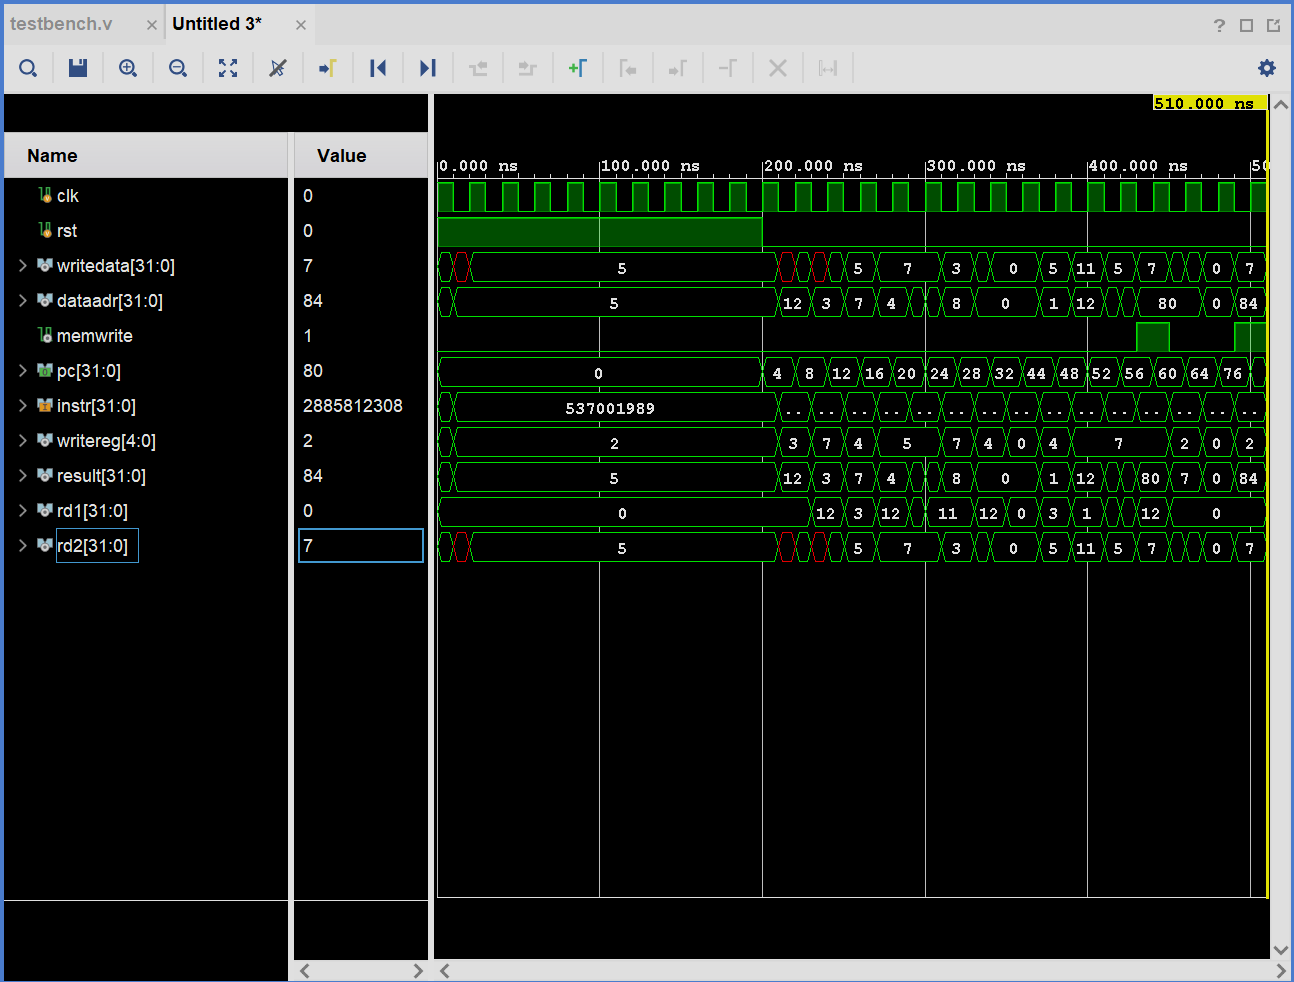
\includegraphics[width=\textwidth]{image/wave.png}
    \caption{单周期CPU仿真波形图（pc、instr、rs、rt、rd、result）}\label{fig:wave}
\end{figure}

\subsection{控制台输出}
图\ref{fig:console}为仿真结束时Tcl控制台截图。testbench.v在negedge clk时检测到dataadr=84（0x54）且writedata=7，与mipstest程序预期最终状态完全一致，控制台打印``Simulation succeeded''，验证了CPU正确实现了全部十条指令。

\begin{figure}[htbp]
    \centering
    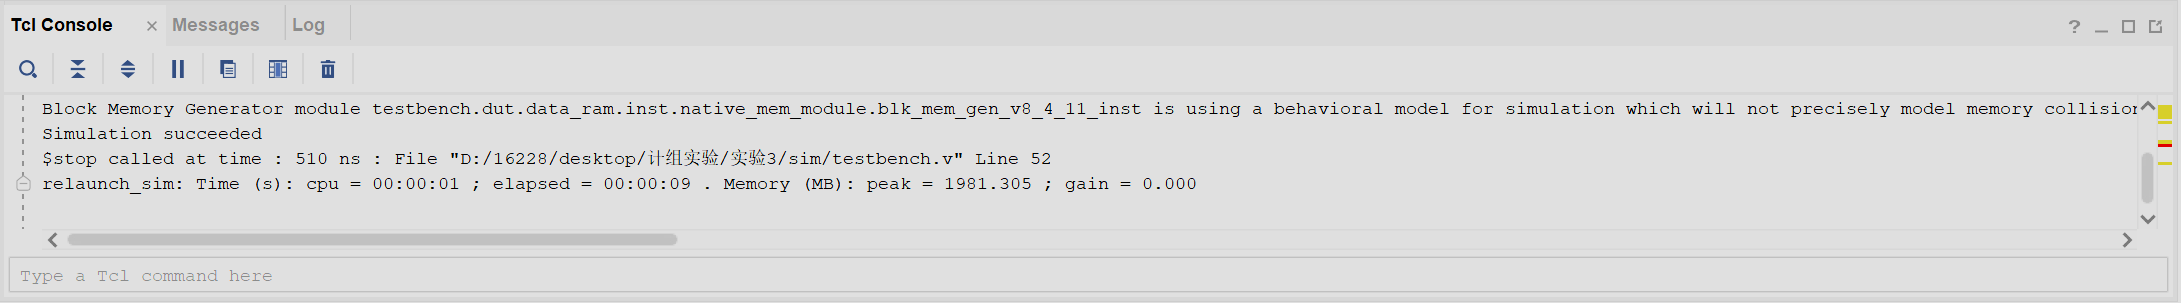
\includegraphics[width=0.85\textwidth]{image/console.png}
    \caption{仿真控制台打印输出}\label{fig:console}
\end{figure}

\subsection{结果分析}
单周期MIPS CPU成功实现了add、sub、and、or、slt（R型）、addi、lw、sw、beq、j共十条指令的数据通路与控制逻辑。testbench程序（mipstest.asm）涵盖所有指令类型，包括两次beq（一次不跳转、一次跳转）、一次j跳转、sw写内存与lw读内存的验证，最终输出结果符合预期，证明数据通路各模块连接正确，控制信号译码无误。上板验收程序（sum100）采用addi、add、beq、j实现1累加到100的循环，最终\$s0=5050（0x13BA），七段数码管显示``13bA''。
\end{document}
